\documentclass[compress]{beamer}
\usetheme{Warsaw}

\usepackage[dutch]{babel}

\usepackage[utf8]{inputenc}
\usepackage{amsmath}
\usepackage{amssymb}
\usepackage{txfonts}
\usepackage{graphicx, import}
\usepackage{csquotes}
\usepackage[backend=biber, style=ieee]{biblatex}
\usepackage{pgfplots}
\usepackage{siunitx}
\usepackage{caption}
\usepackage{subcaption}
\usepackage{tikz}
\usepackage{wrapfig}

% \RequirePackage[left=2cm,right=2cm,top=2.2cm,bottom=4cm]{geometry}
% \RequirePackage[pdftex,pdfpagelabels,bookmarks,hyperindex,hyperfigures,hidelinks]{hyperref}
% \RequirePackage{listings}  % for code
\usepackage{xcolor} % needs to be after listings
% \usefonttheme[onlymath]{serif}

\graphicspath{ {img/} }


\institute{Groep 7}
\date{\today}

\begin{document}

\title{pH meten met een ISFET}
\subtitle{Sensor modules}
\author[Tycho Jöbsis \and Jochem Leijenhorst \and Illya Ustenko]{
    {
        % %\section*{\hspace*{l}}
        \begin{tabular}{ll}
            Tycho Jöbsis        & (500845792)\tabularnewline
            Jochem Leijenhorst  & (500855372)\tabularnewline
            Illya Ustenko       & (500845492)\tabularnewline
        \end{tabular}
    }
}

\begin{frame}
    \titlepage
\end{frame}

% \begin{frame}
%     \frametitle{Inhoudsopgave}\tableofcontents
% \end{frame} 

\begin{frame}
    \frametitle{Opdracht}

    \begin{itemize}
        \item Onderzoek naar drinkwaterproductie
        \item pH meten 
        \begin{itemize}
            \item Nauwkeurig
            \item Over langere tijd
            \item Naar bestaand base station
        \end{itemize}
    \end{itemize}

\end{frame}


\begin{frame}
    \frametitle{Systeemdiagram}

    \begin{figure}
        \centering
        \includegraphics[width=\textwidth]{toplevelDiagram}
    \end{figure}

\end{frame}

\begin{frame}
    \frametitle{Sensormodule}

    \begin{figure}
        \centering
        \includegraphics[width=\textwidth]{topLevelModuleOnly}
    \end{figure}

\end{frame}

%\subsection*{Eisen}
\begin{frame}
    \frametitle{Systeemeisen}

    \begin{table}[ht]
        \centering
        \begin{tabular}{|l|c c|l|}
            \hline
            Beschrijving                 & Min               & Max   & Eenheid           \\
            \hline 
            Afwijking                    &                   & 0.05  & pH                \\ 
            Bereik                       & 2                 & 10    & pH                \\
            Bandbreedte                  & 10                &       & Hz                \\
            $\mathrm{SNR}_{uit}$         & 36                &       & \qty{}{\decibel}  \\
            Rf afstand                   &                   & 10    & \qty{}{\meter}    \\
            Rf BER                       & $1\times10^{-5}$  &       &                   \\
            Levensduur                   & 48                &       & \qty{}{\hour}     \\
            Gemiddeld gebruikte vermogen &                   & 10    & mW                \\
            Energy harvesting            & $>$ 0             &       & mW                \\
            \hline
        \end{tabular}
        \caption{Systeemspecificaties.}
        \label{tab:systemSpecs}
    \end{table}

\end{frame}



\begin{frame}
    \frametitle{Systeemdiagram}
    
    \begin{figure}
        \centering
        \includegraphics[width=\textwidth]{moduleDiagram.pdf}
    \end{figure}
    
\end{frame}
\begin{frame}
    \frametitle{Signaalverwerking}
    
    \begin{figure}
        \centering
        \includegraphics[width=\textwidth]{signaalverwerkingBlokje}
    \end{figure}

\end{frame}

\begin{frame}
    \frametitle{Signaalverwerking}
    
    \begin{figure}
        \centering
        \includegraphics[width=\textwidth]{analogeBewerkingsFunctie}
    \end{figure}

\end{frame}
\begin{frame}
    \frametitle{Uitleesschakeling}
    
    \only<1>{
        \begin{figure}
            \centering
            \includegraphics[width=\textwidth]{pHBlokje}
        \end{figure}
    }

    \only<2>{
        \begin{figure}
            \centering
            \def\svgwidth{0.6\textwidth}
            \input{ISFETCircuitBest.pdf_tex}
        \end{figure}
    }

\end{frame}

\begin{frame}
    \frametitle{Energie}

    \begin{wrapfigure}{r}{0.5\textwidth}
        \centering
        \def\svgwidth{0.5\textwidth}
        \input{ISFETCircuitBest.pdf_tex}
    \end{wrapfigure}
    
    $P_{statisch} = P_{n,quiescent} + U_{dd}I_{ds}$
    \pause
    \vspace{1cm}

    $U_{dd}=3v3$

    $I_{ds}=50\mu$
    \pause

    $P_{statisch} = P_{n,quiescent} + 165\mu\mathrm{W}$
\end{frame}
\begin{frame}
    \frametitle{ADC}
    
    \begin{figure}
        \centering
        \includegraphics[width=\textwidth]{adcBlock}
    \end{figure}

\end{frame}

\begin{frame}
    \frametitle{Eisen}

    \begin{table}[ht]
        \centering
        \begin{tabular}{l|c|l}
            Symbol      & Waarde & Eenheid\\\hline
            $SNR_{in}$  & 37        & dB\\
            NF          & 3         & dB\\
            $u_{in}$    & 2.5       & mV\\
        \end{tabular}
        \caption{De eisen voor het omzetten van het analoge signaal naar een digitaal signaal.}
        \label{tab:systemSpecADC}
    \end{table}
    
\end{frame}
\begin{frame}
    \frametitle{Minimum aantal bits}
    \centering

    De toelaatbare fout ten gevolge van de eindige resolutie van de ADC
    \begin{equation}\label{eq:calcSpecifiedRmsError}
        \overline{e_{eff}^2}=\left(10^{\frac{NF}{10}}-1\right)\left(\frac{S_{rms}}{10^{\left(SNR+NF\right)/20}}\right)^2
    \end{equation}
    \pause

    Berekenen minimum benodigde ADC resolutie
    \begin{equation}\label{eq:calcNeededQ}
        Q=\sqrt{12\cdot\overline{e_{eff}^2}}
    \end{equation}
    \pause

    Berekenen minimum aantal bits van de ADC op basis van de minimaal benodigde ADC resolutie 
    \begin{equation}\label{eq:calcMinNumberADCbits}
        n=\left\lceil\log_2\left(\frac{1}{Q}+1\right)\right\rceil=14
    \end{equation}

\end{frame}

\begin{frame}
    \frametitle{Sample frequentie}
    \centering
    
    Toelaatbare fout
    \begin{equation}\label{eq:ADCmaxSampleError}
        E=10^{\frac{-NF}{10}}
    \end{equation}
    \pause

    Minimale sample frequentie
    \begin{equation}\label{eq:ADCminFs}
        f_{s,min}=\frac{\pi f_h}{E}= \qty{45}{\hertz}
    \end{equation}

\end{frame}

\subsection{Filter}
Tussen de ADC en de uitleesschakeling van de sensor zit een filter. Dit filter zorgt ervoor dat alle frequenties buiten de bandbreedte weggefilterd worden. Er is gekozen om hiervoor een eerste orde laagdoorlaatfilter te gebruiken.
De schakeling van dit filter is te zien in \cref{fig:filterCircuit}. De kantelfrequentie van het filter ligt aan de waardes van $C$ en $R$, volgens \cref{eq:cutoffFreq}.
\begin{figure}[!htbp]
    \centering
    \def\svgwidth{0.3\textwidth}
    \subsection{Filter}
Tussen de ADC en de uitleesschakeling van de sensor zit een filter. Dit filter zorgt ervoor dat alle frequenties buiten de bandbreedte weggefilterd worden. Er is gekozen om hiervoor een eerste orde laagdoorlaatfilter te gebruiken.
De schakeling van dit filter is te zien in \cref{fig:filterCircuit}. De kantelfrequentie van het filter ligt aan de waardes van $C$ en $R$, volgens \cref{eq:cutoffFreq}.
\begin{figure}[!htbp]
    \centering
    \def\svgwidth{0.3\textwidth}
    \subsection{Filter}
Tussen de ADC en de uitleesschakeling van de sensor zit een filter. Dit filter zorgt ervoor dat alle frequenties buiten de bandbreedte weggefilterd worden. Er is gekozen om hiervoor een eerste orde laagdoorlaatfilter te gebruiken.
De schakeling van dit filter is te zien in \cref{fig:filterCircuit}. De kantelfrequentie van het filter ligt aan de waardes van $C$ en $R$, volgens \cref{eq:cutoffFreq}.
\begin{figure}[!htbp]
    \centering
    \def\svgwidth{0.3\textwidth}
    \input{img/filter.pdf_tex}
    \caption{Het eerste-orde filter.}
    \label{fig:filterCircuit}
\end{figure}
\begin{equation} \label{eq:cutoffFreq}
    2\pi f_c = \omega_c = \frac{1}{RC}
    \tagaddtext{[\si{\radian\per\second}]}
\end{equation}

\subsubsection{Ruis}
De spectrale ruisdichtheid aan de ingang van het filter is te berekenen met \cref{eq:filterNoiseDensity}.
De spectrale ruisdichtheid aan de uitgang van het filter is hetzelfde als die van de spanningsdeler in \cref{sec:referenceVoltage}. Deze is te berekenen met \cref{eq:dividerNoise}.


% TODO: BEPAAL OVERDRACHT

% \begin{equation} \label{eq:filterTransfer}
%     H(s) = \frac{1}{1+sRC}
% \end{equation}

\begin{equation} \label{eq:filterNoiseDensity}
    S_{u_{in}} = 4kTR
    \tagaddtext{[\si{\volt\squared\per\hertz}]}
\end{equation}

% De signaal-ruis verhouding aan de uitgang van dit filter is te berekenen met \cref{eq:filterSNR}
% \begin{equation}\label{eq:filterSNR}
%     \mathrm{SNR} = 20\log\left(U_{out,min}\sqrt{\frac{C}{kT}}\right)
%     \tagaddtext{[\si{\decibel}]}
% \end{equation}

\subsubsection{Vermogen}
Het vermogensverbruik van het filter is te berekenen met \cref{eq:filterPowerLaplace}.
\begin{equation} \label{eq:filterPowerLaplace}
    P = \frac{U_{in,max}^2}{\left|R + \frac{1}{sC}\right|}
    \tagaddtext{[\si{\watt}]}
\end{equation}
Omdat volgens \cref{eq:cutoffFreq} $R$ te definiëren is in $\omega_c$ en $C$, volgt hieruit \cref{eq:filterPower}.
\begin{equation} \label{eq:filterPower}
    P = \frac{1}{2}\omega_cCU_{in,max}^2
    \tagaddtext{[\si{\watt}]}
\end{equation}
In deze formule is te zien dat het vermogensverbruik lineair evenredig is met de condensatorwaarde. Om het vermogensverbruik te minimaliseren moet dus een zo klein mogelijke condensatorwaarde gekozen worden. Aangezien de noise-figure van dit filter maximaal 3dB mag zijn, mag dit filter maximaal evenveel spanningsruis genereren als het systeem ervoor. Hieruit volgt \cref{eq:filterCapMin}, waarmee de minimale condensatorwaarde te berekenen is. Hierbij is $u_{n,in}$ de ruisspanning aan de ingang van het filter.
\begin{equation} \label{eq:filterCapMin}
    C_{min} = \frac{kT}{u_{n,in}^2}
    \tagaddtext{[\si{\farad}]}
\end{equation}
    \caption{Het eerste-orde filter.}
    \label{fig:filterCircuit}
\end{figure}
\begin{equation} \label{eq:cutoffFreq}
    2\pi f_c = \omega_c = \frac{1}{RC}
    \tagaddtext{[\si{\radian\per\second}]}
\end{equation}

\subsubsection{Ruis}
De spectrale ruisdichtheid aan de ingang van het filter is te berekenen met \cref{eq:filterNoiseDensity}.
De spectrale ruisdichtheid aan de uitgang van het filter is hetzelfde als die van de spanningsdeler in \cref{sec:referenceVoltage}. Deze is te berekenen met \cref{eq:dividerNoise}.


% TODO: BEPAAL OVERDRACHT

% \begin{equation} \label{eq:filterTransfer}
%     H(s) = \frac{1}{1+sRC}
% \end{equation}

\begin{equation} \label{eq:filterNoiseDensity}
    S_{u_{in}} = 4kTR
    \tagaddtext{[\si{\volt\squared\per\hertz}]}
\end{equation}

% De signaal-ruis verhouding aan de uitgang van dit filter is te berekenen met \cref{eq:filterSNR}
% \begin{equation}\label{eq:filterSNR}
%     \mathrm{SNR} = 20\log\left(U_{out,min}\sqrt{\frac{C}{kT}}\right)
%     \tagaddtext{[\si{\decibel}]}
% \end{equation}

\subsubsection{Vermogen}
Het vermogensverbruik van het filter is te berekenen met \cref{eq:filterPowerLaplace}.
\begin{equation} \label{eq:filterPowerLaplace}
    P = \frac{U_{in,max}^2}{\left|R + \frac{1}{sC}\right|}
    \tagaddtext{[\si{\watt}]}
\end{equation}
Omdat volgens \cref{eq:cutoffFreq} $R$ te definiëren is in $\omega_c$ en $C$, volgt hieruit \cref{eq:filterPower}.
\begin{equation} \label{eq:filterPower}
    P = \frac{1}{2}\omega_cCU_{in,max}^2
    \tagaddtext{[\si{\watt}]}
\end{equation}
In deze formule is te zien dat het vermogensverbruik lineair evenredig is met de condensatorwaarde. Om het vermogensverbruik te minimaliseren moet dus een zo klein mogelijke condensatorwaarde gekozen worden. Aangezien de noise-figure van dit filter maximaal 3dB mag zijn, mag dit filter maximaal evenveel spanningsruis genereren als het systeem ervoor. Hieruit volgt \cref{eq:filterCapMin}, waarmee de minimale condensatorwaarde te berekenen is. Hierbij is $u_{n,in}$ de ruisspanning aan de ingang van het filter.
\begin{equation} \label{eq:filterCapMin}
    C_{min} = \frac{kT}{u_{n,in}^2}
    \tagaddtext{[\si{\farad}]}
\end{equation}
    \caption{Het eerste-orde filter.}
    \label{fig:filterCircuit}
\end{figure}
\begin{equation} \label{eq:cutoffFreq}
    2\pi f_c = \omega_c = \frac{1}{RC}
    \tagaddtext{[\si{\radian\per\second}]}
\end{equation}

\subsubsection{Ruis}
De spectrale ruisdichtheid aan de ingang van het filter is te berekenen met \cref{eq:filterNoiseDensity}.
De spectrale ruisdichtheid aan de uitgang van het filter is hetzelfde als die van de spanningsdeler in \cref{sec:referenceVoltage}. Deze is te berekenen met \cref{eq:dividerNoise}.


% TODO: BEPAAL OVERDRACHT

% \begin{equation} \label{eq:filterTransfer}
%     H(s) = \frac{1}{1+sRC}
% \end{equation}

\begin{equation} \label{eq:filterNoiseDensity}
    S_{u_{in}} = 4kTR
    \tagaddtext{[\si{\volt\squared\per\hertz}]}
\end{equation}

% De signaal-ruis verhouding aan de uitgang van dit filter is te berekenen met \cref{eq:filterSNR}
% \begin{equation}\label{eq:filterSNR}
%     \mathrm{SNR} = 20\log\left(U_{out,min}\sqrt{\frac{C}{kT}}\right)
%     \tagaddtext{[\si{\decibel}]}
% \end{equation}

\subsubsection{Vermogen}
Het vermogensverbruik van het filter is te berekenen met \cref{eq:filterPowerLaplace}.
\begin{equation} \label{eq:filterPowerLaplace}
    P = \frac{U_{in,max}^2}{\left|R + \frac{1}{sC}\right|}
    \tagaddtext{[\si{\watt}]}
\end{equation}
Omdat volgens \cref{eq:cutoffFreq} $R$ te definiëren is in $\omega_c$ en $C$, volgt hieruit \cref{eq:filterPower}.
\begin{equation} \label{eq:filterPower}
    P = \frac{1}{2}\omega_cCU_{in,max}^2
    \tagaddtext{[\si{\watt}]}
\end{equation}
In deze formule is te zien dat het vermogensverbruik lineair evenredig is met de condensatorwaarde. Om het vermogensverbruik te minimaliseren moet dus een zo klein mogelijke condensatorwaarde gekozen worden. Aangezien de noise-figure van dit filter maximaal 3dB mag zijn, mag dit filter maximaal evenveel spanningsruis genereren als het systeem ervoor. Hieruit volgt \cref{eq:filterCapMin}, waarmee de minimale condensatorwaarde te berekenen is. Hierbij is $u_{n,in}$ de ruisspanning aan de ingang van het filter.
\begin{equation} \label{eq:filterCapMin}
    C_{min} = \frac{kT}{u_{n,in}^2}
    \tagaddtext{[\si{\farad}]}
\end{equation}
\subsection{Digitale signaalbewerking}\label{sec:digitaal}

Voorbij de twee signaalverwerkingspaden van de pH waarde en de temperatuur, komt een digitaal signaalverwerkingsblok. Dit blok combineert de twee signalen en rekent deze om naar een pH waarde.
\begin{figure}[!htbp]
    \centering
    \includegraphics[width=0.95\textwidth]{signaalverwerking_digitaal}
    \caption{Waar de digitale signaalbewerking zich bevind in het blokschema van de signaalverwerking in \cref{fig:analogeBewerkingsFunctie}.}
    \label{fig:digitaalInSchema}
\end{figure}

Dit wordt gedaan door middel van een aantal berekeningen. Deze berekeningen zetten de door de ADC gemeten spanningen om naar een pH waarde. Hiervoor zijn een aantal kalibratiewaardes nodig, zoals besproken in \cref{sec:werkingISFET}. Het digitale gedeelte heeft als ingang een temperatuurafhankelijke spanning $U_T$ en een pH-afhankelijke spanning $U_{pH}$. Dit is te zien in \cref{fig:digitaleBewerkingsFunctie}. Beide van deze spanningen zijn de ruwe ADC waardes die gemeten worden, en hebben dus de hoogst mogelijke resolutie, namelijk de resolutie van de ADC. Voor beide van deze waardes zal de eenheid `bit' gebruikt worden.

Om op de uiteindelijk pH waarde te komen, wordt van de pH-afhankelijke spanning de pH-afhankelijke kalibratiespanning afgetrokken. Vervolgens wordt hier $\frac{pH_{kal}}{C_{pH}}$ bij opgeteld. Op deze manier kan er zo lang mogelijk met integers gewerkt worden die dezelfde resolutie hebben als de ingangs-ADC waarde. Het resultaat wordt vervolgens vermenigvuldigd met $C_{pH}$. Dit is de gevoeligheid van de sensor, in pH/bit.

Om de temperatuurafwijking te berekenen, wordt eerst van de temperatuurafhankelijke spanning $U_T$ de temperatuurafhankelijke kalibratiespanning $U_{T,kal}$ afgetrokken. Vervolgens wordt dit vermenigvuldigt met constante $C_T$. $C_T$ is de temperatuurafhankelijkheid van de pH-sensor, in pH/bit. Deze waarde kan afgeleid worden met de temperatuurafhankelijkheid van de pH-sensor die in de datasheet gegeven wordt in mV/K \cite{isfet}.

\begin{figure}[!htbp]
    \centering
    \includegraphics[width=0.95\textwidth]{digitaleBewerkingsFunctie}
    \caption{Het digitale gedeelte van de signaalbewerking.}
    \label{fig:digitaleBewerkingsFunctie}
\end{figure}
\begin{frame}
    \frametitle{Ontvangstgevoeligheid}

    \begin{table}
        \centering
        \begin{tabular}{l|c}
            Eigenschap & Waarde \\\hline
            BER & $1\times10^{-5}$ \\
            $\Delta N$ & -105 dBm \\
            Noise Figure & 12.6 dB \\
            Modulatie & GFSK \\
        \end{tabular}
        \caption{Eigenschappen van de ontvanger op het basisstation.}
    \end{table}

    \pause 

    $S_{or}=-57$ dBm bij B=\qty{1}{\mega\hertz}

    $S_{or}=-54$ dBm bij B=\qty{2}{\mega\hertz}

\end{frame}

\begin{frame}
    \frametitle{Minimum zendvermogen}

    \begin{table}
        \centering
        \begin{tabular}{l|c}
            Eigenschap & Waarde \\\hline
            Afstand & \qty{10}{\meter} \\
            Hoogte & \qty{1}{\meter} \\
        \end{tabular}
        \caption{Antenne plaatsing.}
    \end{table}

    Path loss = 53.2 dB

    \pause

    $\Rightarrow$

    $P_{z}=-4$dBm bij B=\qty{1}{\mega\hertz}

    $P_{z}=-1$dBm bij B=\qty{2}{\mega\hertz}
\end{frame}

\begin{frame}
    \frametitle{Energie en gemiddeld vermogen}

    Energie kosten per verzonden pakket:
    \begin{equation*}
        E_{z,p}=\frac{l}{DR}P_z
    \end{equation*}

    \pause

    $E_{z,p}=$\qty{117.8}{\nano\joule} bij B=\qty{1}{\mega\hertz}

    $E_{z,p}=$\qty{117.6}{\nano\joule} bij B=\qty{2}{\mega\hertz}

    \pause

    \vspace{1cm}
    $\overline{P_z}=E_{z,p}f_s$ $\Rightarrow$ \qty{7.1}{\micro\watt} in geval van een bandbreedte van \qty{2}{\mega\hertz}

\end{frame}
\section{Energie}
    \begin{frame}
        \frametitle{<title>}
    
        
    
    \end{frame}

% %\section{Sensor data naar pH omzetten}

%\subsection*{Uitlezen ISFET}

    \begin{frame}
        \frametitle{Principe schakeling}
    
        \begin{figure}
            \centering
            \def\svgwidth{0.6\textwidth}
            \input{ISFETCircuitBest.pdf_tex}
        \end{figure}
    
    \end{frame}
    

    

    %\subsection*{Berekenen pH}
    
% \section{Energie}
    \begin{frame}
        \frametitle{<title>}
    
        
    
    \end{frame}
% \section{Vragen}
\begin{frame}
    \frametitle{Vragen?}
    
    \centering
    Zijn er nog vragen?

\end{frame}

\begin{frame}
    \frametitle{Bare metal vs RTOS}
    \includegraphics[scale=0.2]{RTOS_werking.png}
    bron foto: academy.nordicsemi.com
\end{frame}

\begin{frame}
    \frametitle{Bare metal vs RTOS}
    Bare-metal
    Voordelen:
    \begin{itemize}
        \item meer efficient
        \item minder geheugen
        \item kan sneller werken
    \end{itemize}
    \vspace{0.5cm}
    Nadelen:
    \begin{itemize}
        \item complexere architectuur
        \item werkt op een type microcontroller
        \item door complexiteit kan minder snel zijn dan RTOS
    \end{itemize}
    \vspace{0.5cm}
    Beiden hebben ISR's.
\end{frame}


\begin{frame}
    \frametitle{Referentiespanning}
    
    \only<1>{
        \begin{figure}
            \centering
            \includegraphics[width=\textwidth]{referenceBlock.pdf}
        \end{figure}
    }

    \only<2>{
        \begin{figure}
            \centering
            \def\svgwidth{0.6\textwidth}
            \subsection{Spanningsreferentie}\label{sec:referenceVoltage}

De ISFET uitleesschakeling heeft een spanningsreferentie nodig om te werken. Deze spanningsreferentie kan op meerdere manieren gegenereerd worden.
% TODO: Vertel misschien over andere methoden.
Uiteindelijk is er een spanningsdeler gekozen om de spanningsreferentie mee te implementeren. De schakeling van deze spanningsdeler is te zien in \autoref{fig:divider}.
De condensator wordt gebruikt om ruis te verminderen op hogere frequenties, en dient ook als filter voor hoogfrequente fouten in de voedingsspanning.

\begin{figure}[ht]
    \centering
    \def\svgwidth{0.5\textwidth}
    \subsection{Spanningsreferentie}\label{sec:referenceVoltage}

De ISFET uitleesschakeling heeft een spanningsreferentie nodig om te werken. Deze spanningsreferentie kan op meerdere manieren gegenereerd worden.
% TODO: Vertel misschien over andere methoden.
Uiteindelijk is er een spanningsdeler gekozen om de spanningsreferentie mee te implementeren. De schakeling van deze spanningsdeler is te zien in \autoref{fig:divider}.
De condensator wordt gebruikt om ruis te verminderen op hogere frequenties, en dient ook als filter voor hoogfrequente fouten in de voedingsspanning.

\begin{figure}[ht]
    \centering
    \def\svgwidth{0.5\textwidth}
    \input{img/divider.pdf_tex}
    \caption{De schakeling van de spanningsdeler die dient als spanningsreferentie.}
    \label{fig:divider}
\end{figure}

\noindent
De overdracht van deze spanningsdeler is te vinden in \autoref{eq:dividerTransfer}.
\begin{equation}\label{eq:dividerTransfer}
    H(s) = \frac{U_{ref}(s)}{U_{dd}(s)} = \frac{R_2}{R_1 + R_2 + R_2Cs}
\end{equation}

\noindent
Het vermogen dat de spanningsdeler dissipeert, kan met \autoref{eq:dividerPower} berekend worden.
\begin{equation}\label{eq:dividerPower}
    P(s) = U_{dd}(s)^2\frac{1+R_2Cs}{R_1 + R_2 + R_1R_2Cs}
\end{equation}
Met een constante DC ingangsspanning kan dit vereenvoudigd worden naar \autoref{eq:dividerPowerSimple}.
\begin{equation}\label{eq:dividerPowerSimple}
    P = \frac{U_{dd}^2}{R_1 + R_2}
\end{equation}

\noindent
Om de ruis van deze schakeling te berekenen moet een aantal stappen genomen worden. Aangezien de ingangsbron $U_{dd}$ een spanningsbron is, kan deze als kortsluiting genomen worden. Op deze manier kunnen de twee weerstanden parallel genomen worden, en verandert de schakeling in een simpel RC filter. In \autoref{fig:dividerNoise} is deze omgebouwde schakeling te zien.

\begin{figure}[ht]
    \centering
    \def\svgwidth{0.35\textwidth}
    \input{img/dividerNoise.pdf_tex}
    \caption{De omgebouwde schakeling om ruis mee te berekenen.}
    \label{fig:dividerNoise}
\end{figure}

\noindent
Voor de spectrale spanningsruisdichtheid aan de uitgang $U_{ref}$ kan \autoref{eq:dividerNoiseLaplace} worden opgesteld.
\begin{equation}\label{eq:dividerNoiseLaplace}
    S_{n,u_{ref}} = 4kTR_e\left(\frac{1}{1 + R_eCs}\right)^2
\end{equation}
Wanneer de absolute waarde van de ruis wordt genomen, kan deze over de bandbreedte geïntegreerd worden. Dit resulteert in \autoref{eq:dividerNoiseInt}.
\begin{equation}\label{eq:dividerNoiseInt}
    u_{n,ref}^2 = \int_{\omega_l}^{\omega_h} 4kTR_e\left(\frac{1}{\sqrt{1 + (R_eC\omega)^2}}\right)^2 d\omega
\end{equation}
Het integraal van deze formule komt uit op \autoref{eq:dividerNoiseIntegrated}.
\begin{equation}\label{eq:dividerNoiseIntegrated}
    u_{n,ref}^2 = \frac{4kT}{C}\left[\arctan(R_eC\omega_h) - \arctan(R_eC\omega_l)\right]
\end{equation}

Zolang de spanning stabiel is hoeft de referentie geen exact gedefinieerde spanning te hebben. Dit is omdat de ADC die de waarde van de sensor gaat uitlezen deze referentiespanning ook als referentie zal gebruiken. De waarde moet echter ergens rond de 1.1V zitten, om de stroombron te laten werken.
In \autoref{sec:currentSource} is hier meer over te lezen.
Aangezien de ingangsspanning 1.8V is, zal de DC overdracht $1.1 / 1.8 = \frac{11}{18}$ zijn. Hieruit komt de weerstandsverhouding in \autoref{eq:dividerResistors}.
\begin{equation}\label{eq:dividerResistors}
    \frac{R_1}{R_2} = \frac{7}{11}
\end{equation}
Een hogere $R_1$ zorgt voor een lager vermogensverbruik, maar ook een hogere ruis. Dit is te zien in \autoref{fig:dividerPlots}.

\begin{figure}
    \centering
    \begin{subfigure}[b]{0.45\textwidth}
        \centering
        \input{plots/dividerNoise}
        \caption{Spanningsruis}
        \label{fig:dividerNoisePlot}
    \end{subfigure}
    \hfill
    \begin{subfigure}[b]{0.45\textwidth}
        \centering
        \input{plots/dividerPower}
        \caption{Vermogensverbruik}
        \label{fig:dividerPower}
    \end{subfigure}
    \caption{De ruis en het vermogensverbruik van de spanningsdeler, ten opzichte van de gekozen weerstandswaarde $R_1$.}
    \label{fig:dividerPlots}
\end{figure}
Op $R_1 = 1\si{\mega\ohm}$ en $C = 10\si{\micro\farad}$ is de spanningsruis $u_{n,ref} = 51\si{\nano\volt}$ en het vermogensverbruik $P = 1.3\si{\micro\watt}$. De andere weerstandswaarde is dan $R_2 \approx 1.6 \si{\mega\ohm}$. Deze waardes vallen binnen de specificaties.

[WELKE SPECS??]
    \caption{De schakeling van de spanningsdeler die dient als spanningsreferentie.}
    \label{fig:divider}
\end{figure}

\noindent
De overdracht van deze spanningsdeler is te vinden in \autoref{eq:dividerTransfer}.
\begin{equation}\label{eq:dividerTransfer}
    H(s) = \frac{U_{ref}(s)}{U_{dd}(s)} = \frac{R_2}{R_1 + R_2 + R_2Cs}
\end{equation}

\noindent
Het vermogen dat de spanningsdeler dissipeert, kan met \autoref{eq:dividerPower} berekend worden.
\begin{equation}\label{eq:dividerPower}
    P(s) = U_{dd}(s)^2\frac{1+R_2Cs}{R_1 + R_2 + R_1R_2Cs}
\end{equation}
Met een constante DC ingangsspanning kan dit vereenvoudigd worden naar \autoref{eq:dividerPowerSimple}.
\begin{equation}\label{eq:dividerPowerSimple}
    P = \frac{U_{dd}^2}{R_1 + R_2}
\end{equation}

\noindent
Om de ruis van deze schakeling te berekenen moet een aantal stappen genomen worden. Aangezien de ingangsbron $U_{dd}$ een spanningsbron is, kan deze als kortsluiting genomen worden. Op deze manier kunnen de twee weerstanden parallel genomen worden, en verandert de schakeling in een simpel RC filter. In \autoref{fig:dividerNoise} is deze omgebouwde schakeling te zien.

\begin{figure}[ht]
    \centering
    \def\svgwidth{0.35\textwidth}
    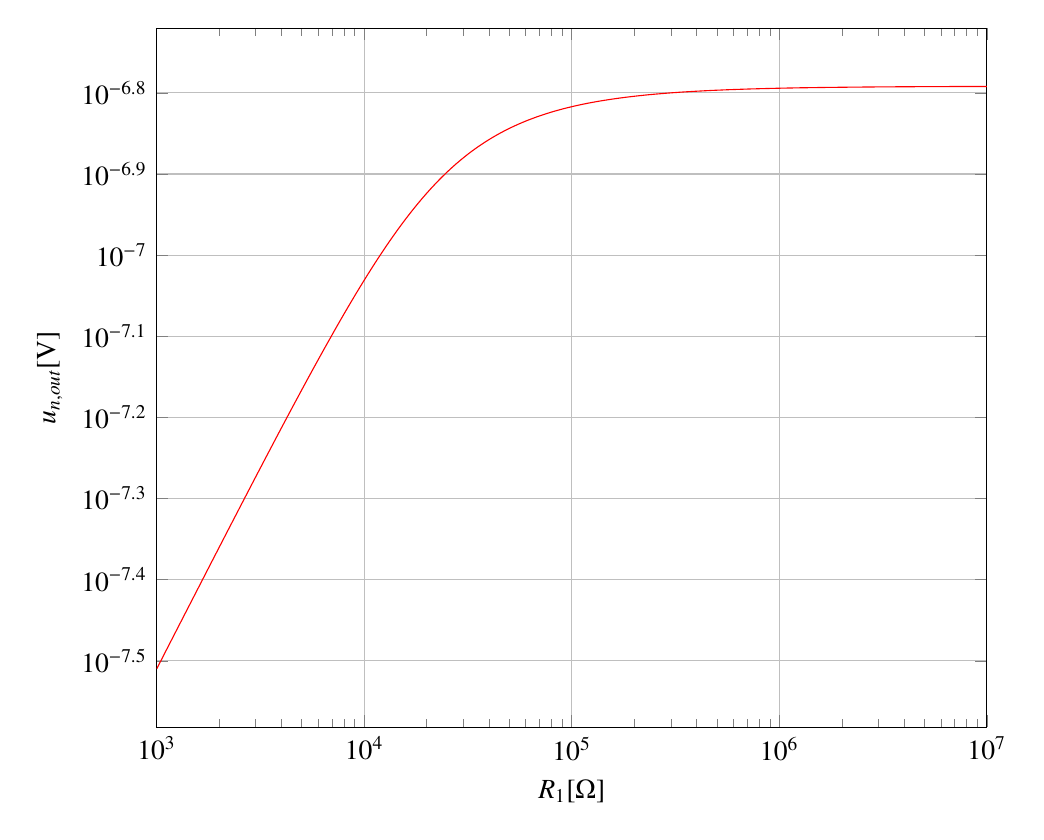
\begin{tikzpicture}
    \pgfplotsset{width=\textwidth}
    \newcommand\BOLZ{1.380649e-23}
    \newcommand\TEMP{300}
    \newcommand\OMEGAC{15*2*pi}
    \newcommand\RESRAT{(7/11)}
    \newcommand\REQU{(1/(1/x + \RESRAT/x))}
    \newcommand\CAP{0.000001}

    \pgfplotsset{set layers}
    \begin{axis}[
        xmode=log,
        ymode=log,
        xlabel={$R_1 [\si{\ohm}]$},
        ylabel={$u_{n,out} [\si{\volt}]$},
        xmin=1e3, xmax=1e7,
        grid=major
    ]

    \addplot [
        red,
        domain=1e3:1e7,
        samples=201
    ]
    {sqrt((4 * \BOLZ * \TEMP / \CAP) * rad(atan(\REQU * \CAP * \OMEGAC)))};
    \end{axis}
\end{tikzpicture}
    \caption{De omgebouwde schakeling om ruis mee te berekenen.}
    \label{fig:dividerNoise}
\end{figure}

\noindent
Voor de spectrale spanningsruisdichtheid aan de uitgang $U_{ref}$ kan \autoref{eq:dividerNoiseLaplace} worden opgesteld.
\begin{equation}\label{eq:dividerNoiseLaplace}
    S_{n,u_{ref}} = 4kTR_e\left(\frac{1}{1 + R_eCs}\right)^2
\end{equation}
Wanneer de absolute waarde van de ruis wordt genomen, kan deze over de bandbreedte geïntegreerd worden. Dit resulteert in \autoref{eq:dividerNoiseInt}.
\begin{equation}\label{eq:dividerNoiseInt}
    u_{n,ref}^2 = \int_{\omega_l}^{\omega_h} 4kTR_e\left(\frac{1}{\sqrt{1 + (R_eC\omega)^2}}\right)^2 d\omega
\end{equation}
Het integraal van deze formule komt uit op \autoref{eq:dividerNoiseIntegrated}.
\begin{equation}\label{eq:dividerNoiseIntegrated}
    u_{n,ref}^2 = \frac{4kT}{C}\left[\arctan(R_eC\omega_h) - \arctan(R_eC\omega_l)\right]
\end{equation}

Zolang de spanning stabiel is hoeft de referentie geen exact gedefinieerde spanning te hebben. Dit is omdat de ADC die de waarde van de sensor gaat uitlezen deze referentiespanning ook als referentie zal gebruiken. De waarde moet echter ergens rond de 1.1V zitten, om de stroombron te laten werken.
In \autoref{sec:currentSource} is hier meer over te lezen.
Aangezien de ingangsspanning 1.8V is, zal de DC overdracht $1.1 / 1.8 = \frac{11}{18}$ zijn. Hieruit komt de weerstandsverhouding in \autoref{eq:dividerResistors}.
\begin{equation}\label{eq:dividerResistors}
    \frac{R_1}{R_2} = \frac{7}{11}
\end{equation}
Een hogere $R_1$ zorgt voor een lager vermogensverbruik, maar ook een hogere ruis. Dit is te zien in \autoref{fig:dividerPlots}.

\begin{figure}
    \centering
    \begin{subfigure}[b]{0.45\textwidth}
        \centering
        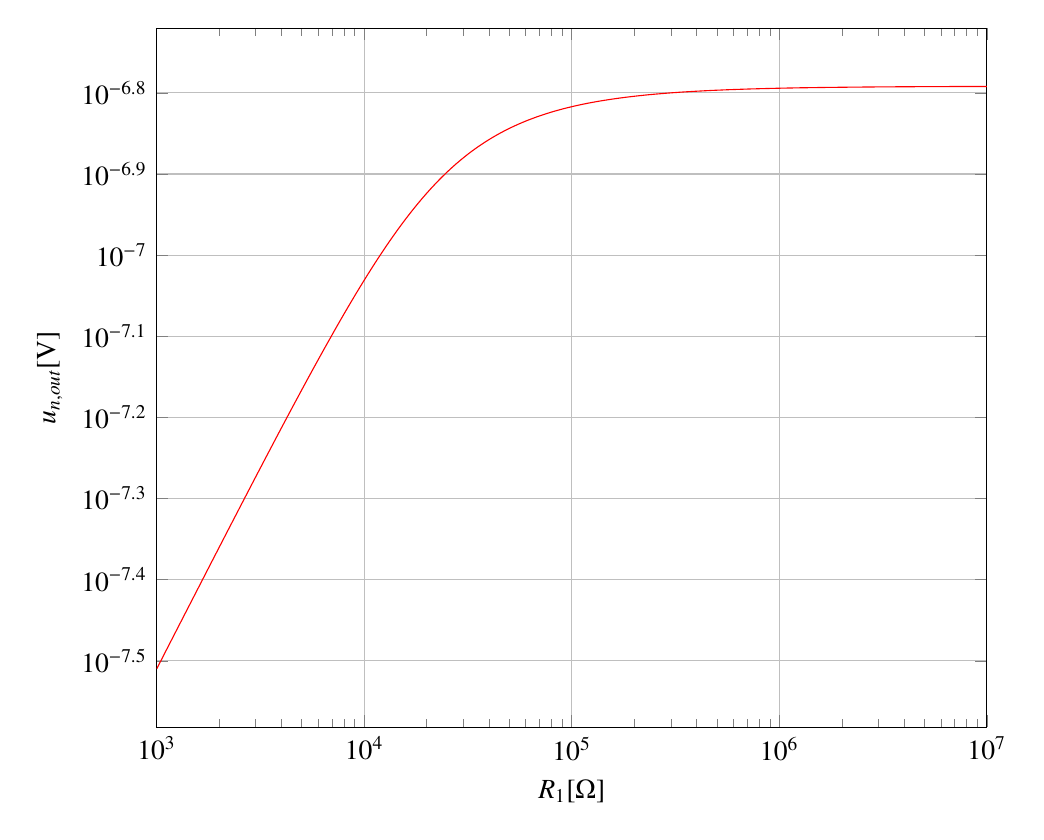
\begin{tikzpicture}
    \pgfplotsset{width=\textwidth}
    \newcommand\BOLZ{1.380649e-23}
    \newcommand\TEMP{300}
    \newcommand\OMEGAC{15*2*pi}
    \newcommand\RESRAT{(7/11)}
    \newcommand\REQU{(1/(1/x + \RESRAT/x))}
    \newcommand\CAP{0.000001}

    \pgfplotsset{set layers}
    \begin{axis}[
        xmode=log,
        ymode=log,
        xlabel={$R_1 [\si{\ohm}]$},
        ylabel={$u_{n,out} [\si{\volt}]$},
        xmin=1e3, xmax=1e7,
        grid=major
    ]

    \addplot [
        red,
        domain=1e3:1e7,
        samples=201
    ]
    {sqrt((4 * \BOLZ * \TEMP / \CAP) * rad(atan(\REQU * \CAP * \OMEGAC)))};
    \end{axis}
\end{tikzpicture}
        \caption{Spanningsruis}
        \label{fig:dividerNoisePlot}
    \end{subfigure}
    \hfill
    \begin{subfigure}[b]{0.45\textwidth}
        \centering
        \begin{tikzpicture}
    \pgfplotsset{width=\textwidth}
    \newcommand\OMEGAC{10*2*pi}
    \newcommand\RESRAT{(7/11)}

    \begin{axis}[
        xmode=log,
        ymode=log,
        xlabel={$R_1 [\si{\ohm}]$},
        ylabel={$P [\si{\watt}]$},
        xmin=1e3, xmax=2e6,
        grid=major
    ]

    \addplot [
        blue,
        domain=1e3:2e6,
        samples=201
    ]
    {1.8 / (x + x/\RESRAT)};
    \end{axis}
\end{tikzpicture}
        \caption{Vermogensverbruik}
        \label{fig:dividerPower}
    \end{subfigure}
    \caption{De ruis en het vermogensverbruik van de spanningsdeler, ten opzichte van de gekozen weerstandswaarde $R_1$.}
    \label{fig:dividerPlots}
\end{figure}
Op $R_1 = 1\si{\mega\ohm}$ en $C = 10\si{\micro\farad}$ is de spanningsruis $u_{n,ref} = 51\si{\nano\volt}$ en het vermogensverbruik $P = 1.3\si{\micro\watt}$. De andere weerstandswaarde is dan $R_2 \approx 1.6 \si{\mega\ohm}$. Deze waardes vallen binnen de specificaties.

[WELKE SPECS??]
        \end{figure}
    }

\end{frame}


\begin{frame}
    \frametitle{Ruis analyse}

    \begin{figure}
        \centering
        \def\svgwidth{0.7\textwidth}
        \input{ISFETCircuitBestNoise.pdf_tex}
    \end{figure}
    \begin{equation*}\label{eq:measureNoiseOut}
        S_{u_{{n,out}}} = \left(S_{u_{{n,ref}}} + S_{u_{{n,n}}} + S_{i_{{n,in}}}\left(Z_{fet} // R\right)^2\right) \cdot H^2(ph)
    \end{equation*}

\end{frame}

\begin{frame}
    \frametitle{Power and harvest schema}
    \centering
    \includegraphics[scale=0.4]{powerAndHarvest2.pdf}
\end{frame}

\begin{frame}
    \frametitle{Efficiency buck only vs buck-boost}
    \centering
    \includegraphics[scale=0.9]{buckvsbuckboost.png}\\
    Efficiency gekozen mode, oranje lijn. Rond 90\%\\
    Bron: LTC3330 datasheet
\end{frame}

\begin{frame}
    \frametitle{Buck-boost swithcing}
    \centering
    \includegraphics[scale=0.9]{buck_boost_switching.png}\\
    Bron: LTC3330 datasheet
\end{frame}

\begin{frame}
    \frametitle{LDO Spanning}
    \centering
    \includegraphics[scale=0.9]{ldo_spannign.png}\\
    Bron: LTC3330 datasheet
\end{frame}

\begin{frame}
    \frametitle{Buck step respone}
    \centering
    \includegraphics[scale=0.9]{buck_step_response.png}\\
    Bron: LTC3330 datasheet
\end{frame}

\begin{frame}
    \frametitle{LDO step respone}
    \centering
    \includegraphics[scale=0.9]{ldo_step.png}\\
    Bron: LTC3330 datasheet
\end{frame}

\begin{frame}
    \frametitle{Sensor uitlees + analog}
    \centering
    \includegraphics[scale=0.3]{sensorBord.png}\\
\end{frame}

\begin{frame}
    \frametitle{Power and Harvest}
    \centering
    \includegraphics[scale=0.18]{powerAndHarvest.png}\\
\end{frame}

\begin{frame}
    \frametitle{Test Ugs Uds}
    \centering
    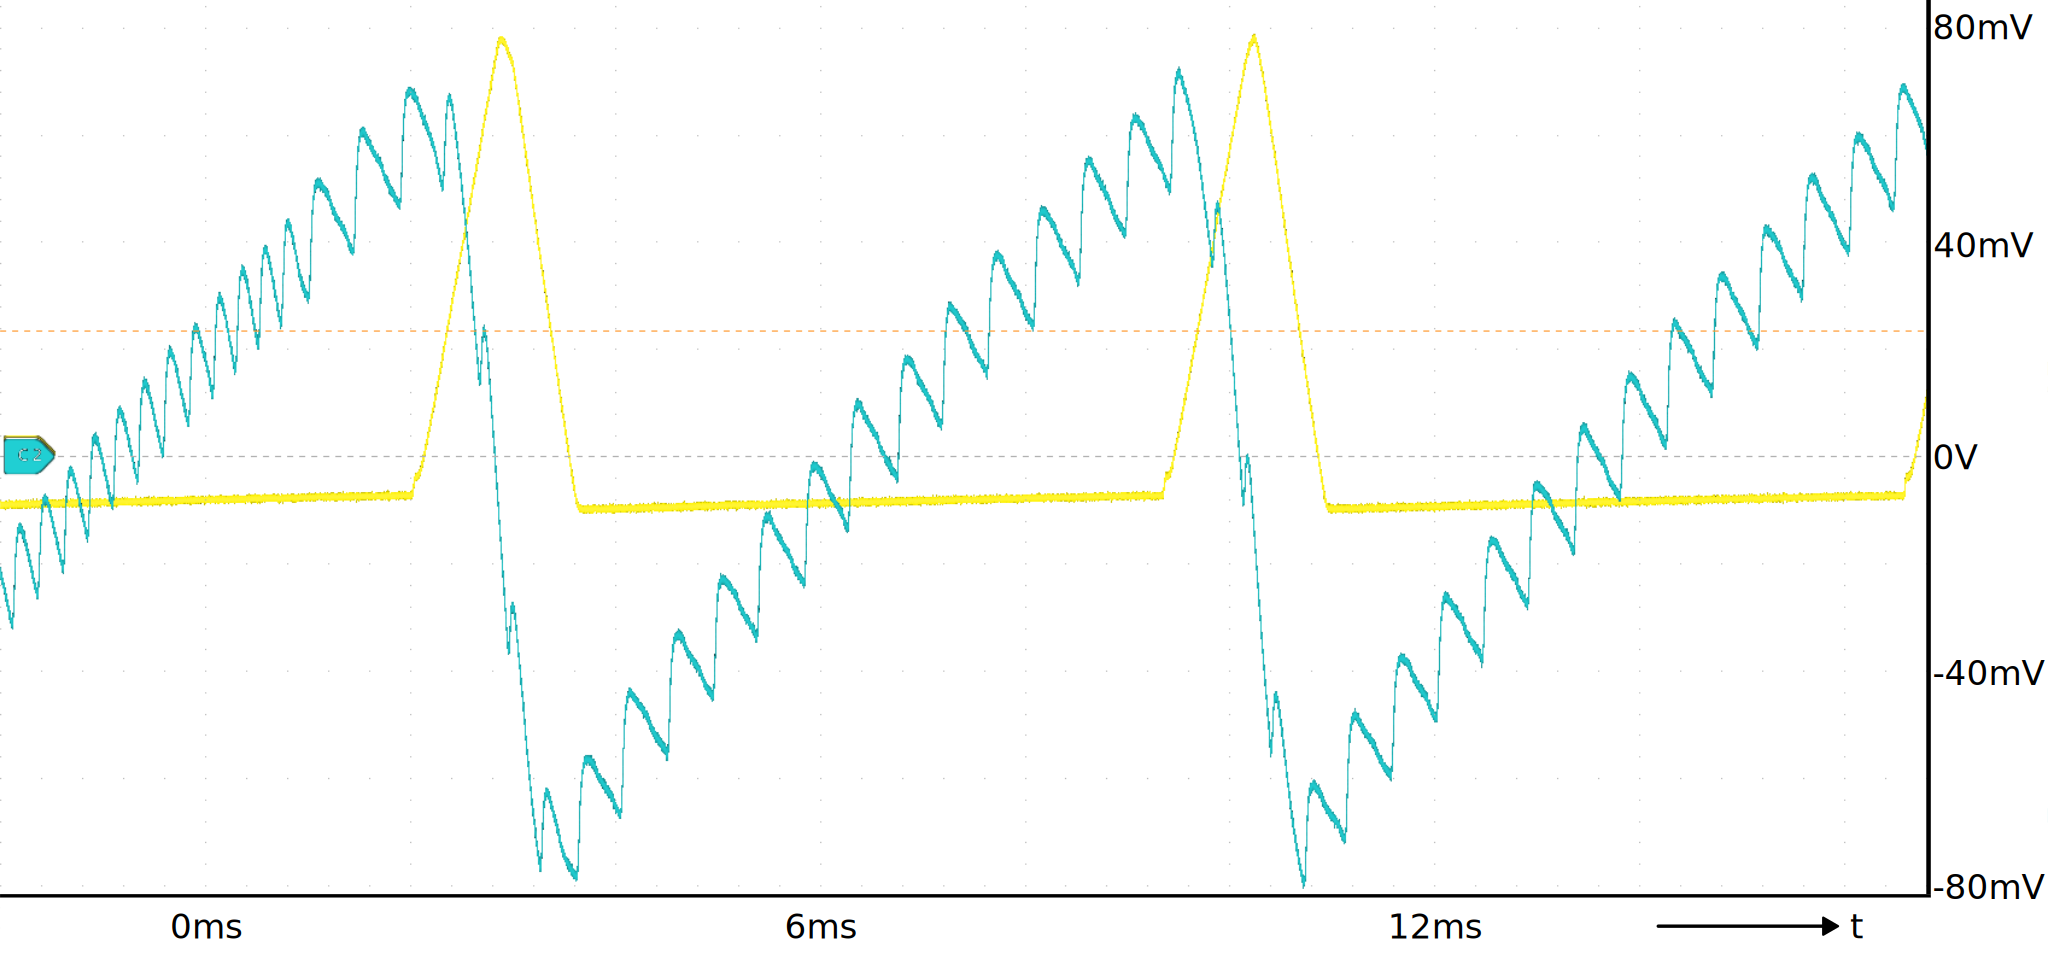
\includegraphics[scale=0.17]{testUgsUds.png}\\
\end{frame}

\begin{frame}
    \frametitle{pH 7 Test}
    \centering
    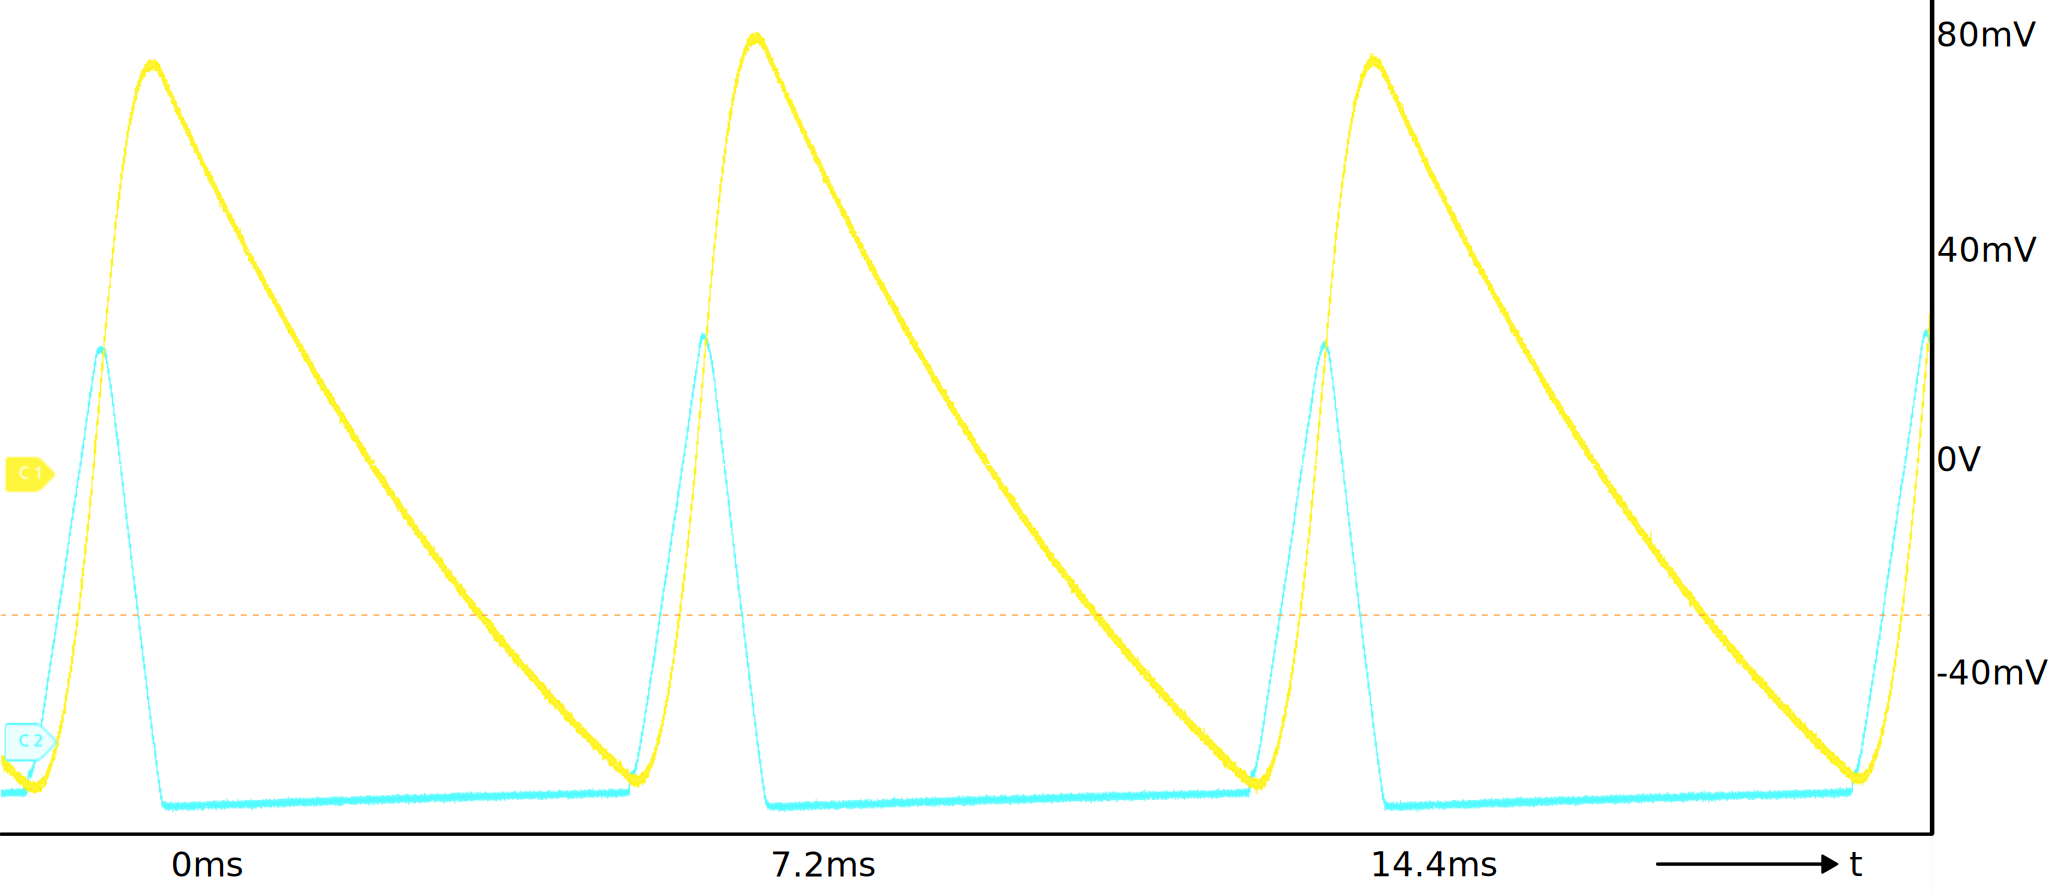
\includegraphics[scale=0.17]{testpH7.png}\\
\end{frame}

\begin{frame}
    \frametitle{pH 4 Test}
    \centering
    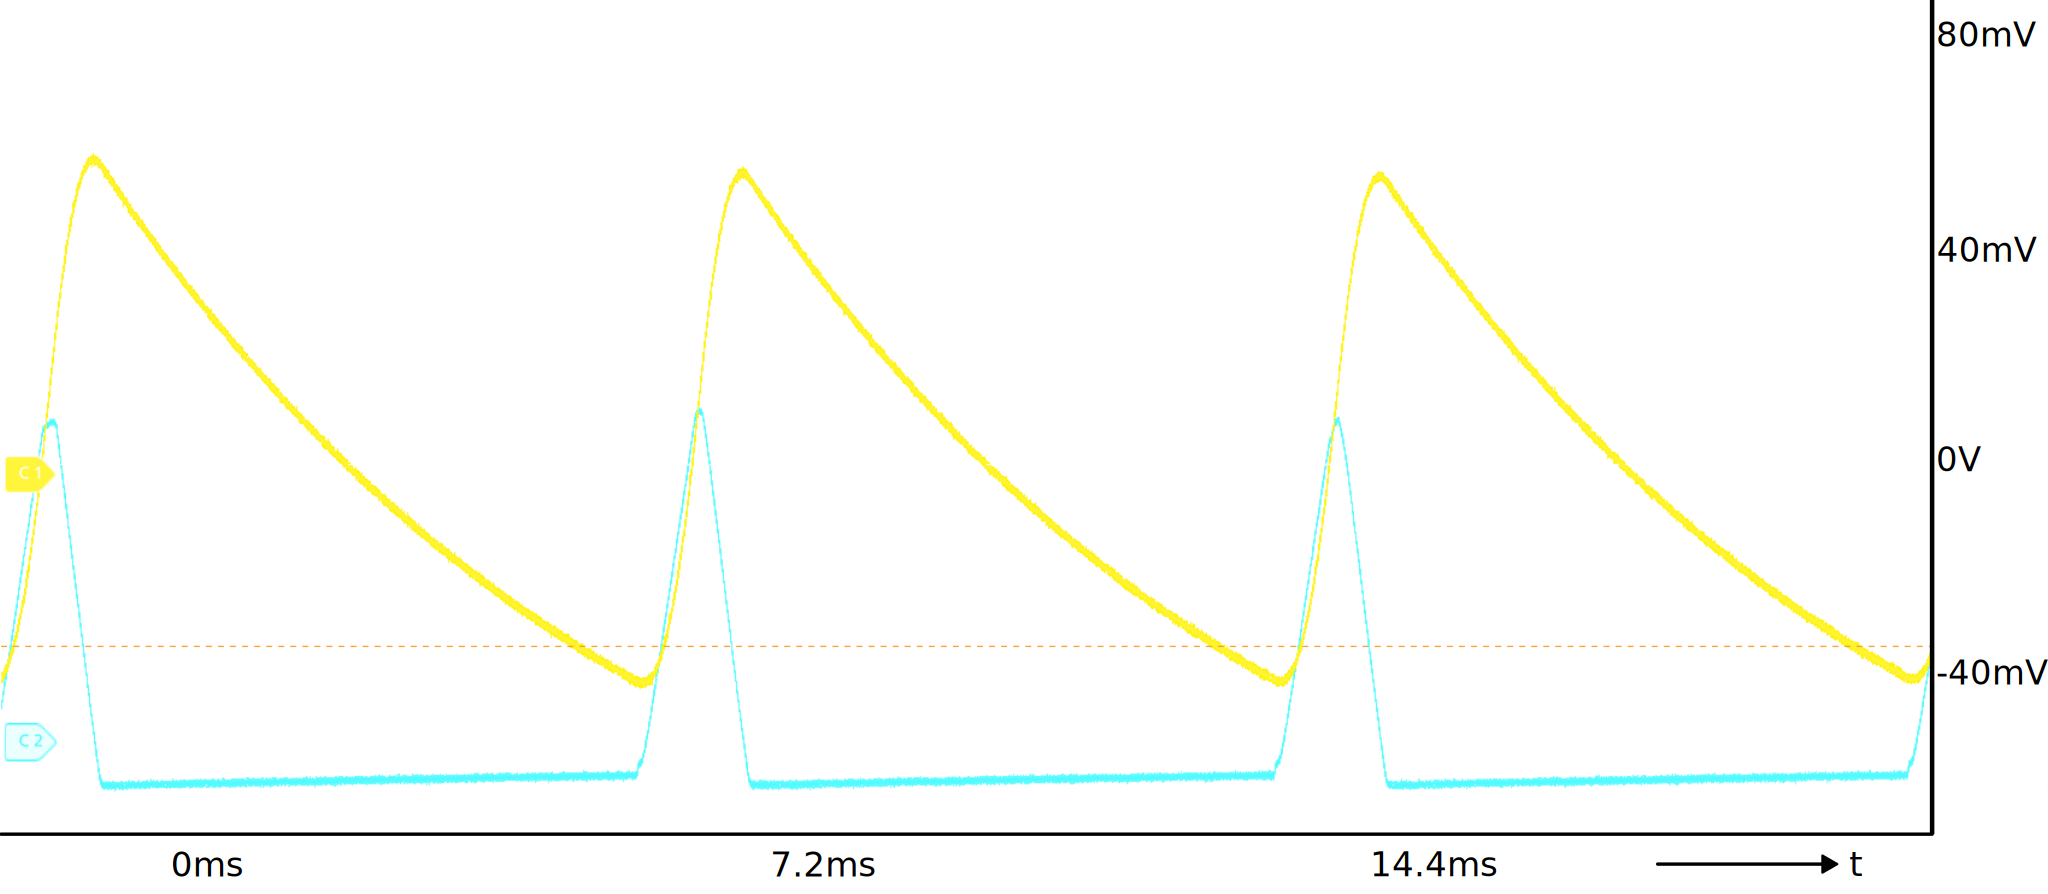
\includegraphics[scale=0.17]{testpH4.png}\\
\end{frame}

\begin{frame}
    \frametitle{Enervery harvesting test opstelling}
    \centering
    \includegraphics[scale=0.4]{energyHarvestingOpstelling.png}\\
\end{frame}


\end{document}